% This file is part of the stream_information project.
% Copyright 2017 the authors. All rights reserved.

% # style notes
% - it is Cram\'er--Rao not Cram\'er-Rao. And yet Fisher-matrix not Fisher--matrix.

\documentclass[modern]{aastex62}

% \usepackage{amsmath}

% typography
\setlength{\parindent}{1.\baselineskip}
% \newcommand{\acronym}[1]{{\small{#1}}}
\newcommand{\package}[1]{\textsl{#1}}
\newcommand{\gaia}{\textsl{Gaia}}

% aastex parameters
% \received{not yet; THIS IS A DRAFT}
%\revised{not yet}
%\accepted{not yet}
% % Adds "Submitted to " the arguement.
% \submitjournal{ApJ}
\shorttitle{GD-1 in Gaia DR2}
\shortauthors{price-whelan \& bonaca}

%@arxiver{}

\begin{document}\sloppy\sloppypar\raggedbottom\frenchspacing % trust me

\title{Gaia DR2 view of the GD-1 stellar stream}

\author[0000-0003-0872-7098]{Adrian~M.~Price-Whelan}
\affiliation{Department of Astrophysical Sciences,
             Princeton University, Princeton, NJ 08544, USA}
\email{adrn@astro.princeton.edu}
\correspondingauthor{Adrian M. Price-Whelan}

\author[0000-0002-7846-9787]{Ana Bonaca}
\affil{Harvard--Smithsonian Center for Astrophysics, Cambridge, MA 02138, USA}


\begin{abstract}\noindent % trust me

\end{abstract}

\keywords{Galaxy: halo --- dark matter}

\section{Introduction}
\label{sec:intro}


\section{Data}
\label{sec:data}

(\citealt{Schlegel:1998, Schlafly:2011}; hereafter SFD)

Maximum $A_G$ is $\approx$0.07 mag in both the under-density and gap regions.

% Notebook: GD1-dust-and-completeness
\begin{figure}[h]
\begin{center}
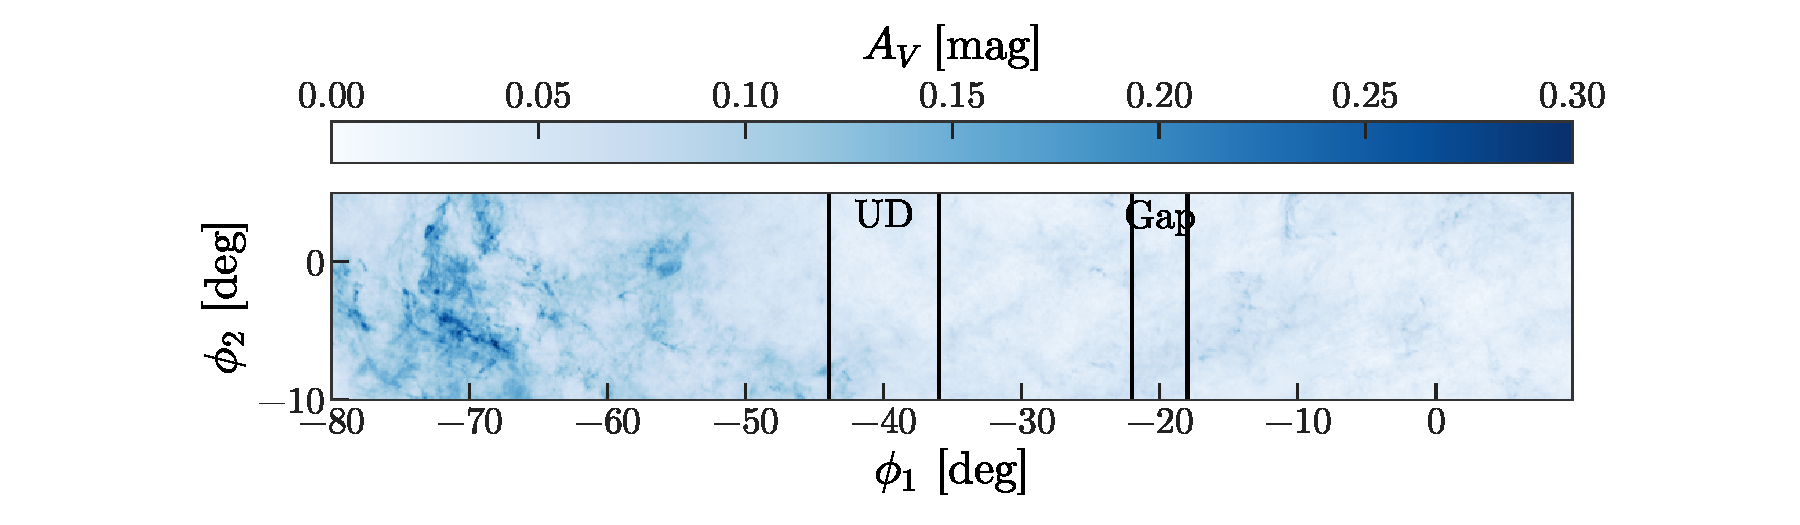
\includegraphics[width=\textwidth]{sfd.pdf}
\end{center}
\caption{%
Colored background shows the \gaia\ $G$-band extinction, $A_G$, in the GD-1
coordinate system.
Vertical lines roughly show the regions identified as the under-density (UD) and
gap.
The maximum extinction in the UD or Gap regions is $\approx$0.07 mag.
\label{fig:sfd}
}
\end{figure}


\section{Results}
\label{sec:results}

\subsection{Global properties}
\label{sec:res_global}

\subsection{Gap}
\label{sec:res_gap}

\subsection{Underdensity}
\label{sec:res_underdensity}


\section{Discussion}
\label{sec:discussion}


\acknowledgements{
thanks: Casey, Geha, Hogg, Spergel, Koposov
CCA for hospitality
AB acknowledges generous support from the Institute for Theory and Computation at Harvard University.
All code used in this work and all results are available at \url{https://github.com/adrn/GD1-DR2}.
}

\software{
    \package{Astropy} \citep{astropy},
    \package{gala} \citep{gala},
    \package{IPython} \citep{ipython},
    \package{matplotlib} \citep{mpl},
    \package{numpy} \citep{numpy},
    \package{scipy} \citep{scipy}
}

\bibliographystyle{aasjournal}
\bibliography{gd1}

\clearpage

\appendix
\section{Completeness check and data validation}
\label{sec:validate}

% % Notebook:
% \begin{figure}[h]
% \begin{center}
% \includegraphics[width=0.7\textwidth]{nvisits.pdf}
% \end{center}
% \caption{%
% TODO
% \label{fig:TODO}
% }
% \end{figure}


\end{document}
